\chapter{Domain Analysis}
General-purpose languages (GPLs) are robust and versatile, but they have weaknesses like everything. Comparing GPLs with general doctors:

\emph{“They are good at solving the first layer of diseases (problems), but they can’t go deep, such as having a full diagnosis of heart disease (domain-related problems)”} \cite{alves}.

Thus DSLs were created to provide a more effective way to address specific problems in a particular domain or industry. Starting with the definition of domain-specific language. \emph{“Domain-specific languages are languages tailored to a specific application domain. They offer substantial gains in expressiveness and ease of use compared with general-purpose programming languages in their domain of application”} \cite{mernik}.
Rather than relying on general-purpose programming languages, which may not be optimized for a specific task or domain, DSLs allow developers to create languages that are tailored to the specific needs of a particular domain. This can result in increased productivity, better code readability, and more efficient code execution \cite{jetbrains}.
Developing a Domain-Specific Language is a challenging task that requires a combination of expertise in both language development and the specific domain the language is intended for. Due to this difficulty, many people who lack the necessary skills and knowledge may delay or altogether avoid the decision to create a DSL. As a result, most DSLs end up being limited to a specific application or library and are never fully realized or implemented. \par


%The first chapter of the project report contains background information about the problem, the associated domain, and the impact the problem has on the identified domain. 
%Also, when knowing the domain, one could establish target groups and perform customer validation in order to justify the relevance of the problem and the need for the project itself. \cite{chicago}

%Also, it is important to represent the project in a comparative analysis in relation to other analogs. 
%By doing this, the project team can emphasize what the analogs lack and what the new solution could improve.


\section{Problem Description and Problem Analysis}

Health should be every human priority. Good health is fundamental to our happiness and well-being, but also it should be a concern for the government since health and the economy are inextricably linked.
A healthy population is essential for sustainable development and a strong macroeconomy. In turn, a strong economy is necessary to generate sufficient resources for health systems. Yet, despite this mutually beneficial relationship, it is often overlooked and health systems expenditure isn’t taken into consideration most of the time. They may support the goal of universal health coverage, but have concerns that spending on health may be a drain on the economy \cite{health}.

The Republic of Moldova has a universal health care system. The financing of healthcare services in the country is based on the principles of fairness and unity, ensuring that everyone has equal access to healthcare services regardless of their financial status. However, over 10\% of the population lacks health insurance coverage \cite{country}. 
The level of transparency of the domestic health system is 36\%, which ranks us among the countries with an unsatisfactory level of transparency.  It is relatively simple to increase transparency by publishing data that institutions have already created and utilized internally \cite{carp}. \par
In order to identify potential issues within the healthcare system that could be addressed or improved, secondary research was conducted. Secondary research involves analyzing and utilizing pre-existing data sources rather than collecting new data through primary research methods. This approach allows for the examination of a large amount of information and can provide insights into current trends, patterns, and potential areas for improvement.

A domain-specific language can be an effective solution to address the lack of system interoperability in healthcare. Healthcare systems often use different data formats and structures, which can make it difficult to share data between systems. By creating a DSL specifically designed for healthcare data, healthcare professionals can standardize the way that data is stored, analyzed, and shared across different systems. This can help to improve interoperability and make it easier for healthcare professionals to access and use patient data from different sources. By using a common language, DSL can help to reduce errors and inconsistencies that can arise when data is transferred between different systems, ultimately improving patient care and outcomes. \par
When it comes to medical results analysis, DSL can be very useful as it can allow healthcare professionals to quickly and accurately analyze large amounts of medical data. \par
Here are some key aspects of using DSL for medical results analysis:

\emph{Accuracy}: Medical data analysis requires a high degree of accuracy to ensure that diagnoses and treatment plans are appropriate. Using a DSL specifically designed for medical data analysis can help ensure that the analysis is accurate and consistent.

\emph{Efficiency}: DSL can help streamline the analysis process by providing a concise and efficient way to process large amounts of medical data. This can save healthcare professionals time and effort, allowing them to focus on other aspects of patient care.

\emph{Customizability}: DSL can be customized to meet the specific needs of different medical specialties. For example, a DSL designed for radiology analysis may have different features than one designed for analyzing blood test results.

\emph{Accessibility}: DSL can make medical data analysis more accessible to healthcare professionals who may not have extensive programming experience. This can help ensure that more healthcare professionals are able to analyze medical data and make informed decisions based on the results.

\emph{Collaboration}: DSL can facilitate collaboration between healthcare professionals by providing a standardized way to analyze medical data. This can help ensure that everyone is using the same methodology and producing consistent results. \par
Overall, using a DSL for medical results analysis can be a powerful tool for healthcare professionals. It can help improve the accuracy and efficiency of medical data analysis while also making it more accessible and customizable.

\section{Similar Solutions}
There are several existing Domain Specific Languages for analyzing medical results, including:\par
\emph{MQL (Medical Query Language)}: MQL is a language designed for querying and analyzing medical data. It provides a way to express complex queries and calculations that involve medical concepts and terminology. MQL allows users to search medical databases for specific data elements, such as laboratory results or diagnosis codes. MQL is commonly used in healthcare analytics and research.

\emph{SPL (Structured Product Labeling)}: SPL is a standard format for sharing medical product information. It includes data elements such as indications, contraindications, and adverse events. SPL is used by pharmaceutical companies to provide product information to regulatory agencies such as the FDA. SPL files can be used by healthcare professionals to access information about medications, including dosing information and potential side effects.

\emph{HL7 FHIR (Fast Healthcare Interoperability Resources)}: FHIR is a standard for exchanging healthcare information electronically. It includes resources for managing patient data, such as observations, conditions, and medications. FHIR is designed to be easy to implement and can be used with web-based technologies such as REST and JSON. FHIR is widely used in electronic health record systems and healthcare data exchange.

\emph{OpenEHR}: OpenEHR is a standard for electronic health records that includes a formal language for representing clinical concepts and data. OpenEHR provides a way to create reusable clinical models that can be used across different healthcare settings. The language used in OpenEHR is designed to be simple and easy to understand, making it accessible to healthcare professionals with limited technical knowledge.

\emph{CQL (Clinical Quality Language)}: CQL is a language for expressing clinical quality measures. It provides a way to define and calculate quality measures based on clinical data. CQL is used by healthcare organizations to measure and improve the quality of care provided to patients. CQL can be used with electronic health records and other healthcare data sources to calculate quality measures.

\emph{Arden Syntax}: Arden Syntax is a DSL for defining clinical decision support rules. It allows healthcare providers to create rules-based systems that can analyze patient data and provide recommendations for diagnosis and treatment.
% \addcontentsline{toc}{section}{Solution Proposal}

\section{Solution Proposal}
Healthcare organizations should look for advanced solutions that support: easy information gathering, real-time data updates, clear data visualization, and simple reporting.

\textbf{MeDSL} wi be designed to facilitate the analysis of medical test results by providing a simple, user-friendly interface that allows clinicians and researchers, even patients to define algorithms for analyzing test results. 
The DSL will support a range of data types, including numerical, categorical, and text data, and provide tools for data visualization and statistical analysis.

To simplify the process of algorithm development, the DSL will include a comprehensive library of pre-defined functions and operators for common data manipulations, such as filtering, aggregation, and transformation.

Additionally, the DSL will be designed to integrate seamlessly with existing Electronic Health Record (EHR) systems and provide secure access to patient data while maintaining patient privacy and confidentiality.

Overall, the proposed DSL aims to provide an intuitive, flexible, and powerful tool for analyzing medical test results, enabling clinicians and researchers to make more informed decisions and improve patient outcomes.

% \vspace{0.5cm}
% { \centering \includegraphics[width=\textwidth]{images/concept.png} }


\vspace{0.5cm}

{ \centering 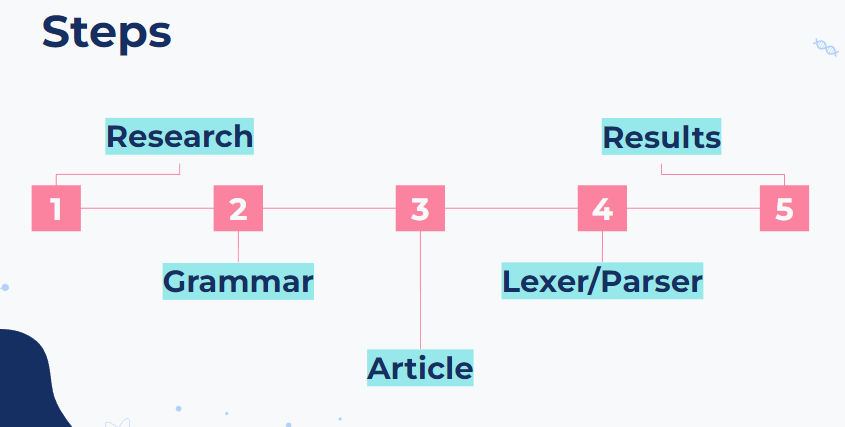
\includegraphics[width=\textwidth]{images/plan.png} }

\section{Target Group and Customer Validation}

In the development of a domain-specific language for analyzing medical results, it is essential to consider the target group and conduct customer validation. The target group for a domain-specific language for analyzing medical results can vary depending on the specific context and purpose of the language. However, in general, the following groups can be considered as potential users:
\begin{enumerate}
\item Medical Professionals: This group includes doctors, nurses, and lab technicians responsible for analyzing medical test results. They have in-depth knowledge and expertise in interpreting test results and making diagnoses, and they are the primary users of the language.

\item Researchers: Researchers in the medical field can also be a potential target group for the language. They may need to analyze large sets of medical data to identify trends, patterns, and potential correlations between test results and specific health conditions.

\item Healthcare Administrators: This group includes hospital administrators and healthcare executives who need to analyze medical data to make informed decisions about healthcare policies, resource allocation, and cost management.

\item Medical Students: Medical students could also be considered as potential users of the language. They may use the language to learn how to analyze medical test results accurately, make diagnoses, and develop treatment plans.

\item Patients: Patients could also benefit from a domain-specific language for analyzing medical results, especially for those who want to understand their test results and communicate more effectively with their healthcare providers.
\end{enumerate}
In summary, the target group for a domain-specific language for analyzing medical results should primarily include medical professionals, researchers, and healthcare administrators. However, considering other potential users such as medical students and patients can also help in developing a more comprehensive and user-friendly language that can serve a broader range of users.

\vspace{0.5cm}
\section{Comparative Analysis}

Here is a comparative analysis of the DSLs for analyzing medical results:
\begin{enumerate}
\item OpenEHR: OpenEHR is a flexible and comprehensive DSL that allows for the creation of standardized electronic health records. It provides a rich set of data types and a standardized data model that can be used to represent clinical data from a wide range of sources. OpenEHR has a well-established community and a growing number of implementations, making it a popular choice for many healthcare providers.

\item HL7 FHIR: HL7 FHIR is a widely adopted standard for exchanging healthcare information electronically. It provides a set of resources and APIs that can be used to develop applications for accessing and analyzing medical data. FHIR is designed to be easy to implement and use, and it has gained widespread adoption among EHR vendors and healthcare providers.

\item Clinical Quality Language (CQL): CQL is a DSL for defining clinical quality measures. It allows for the creation of standardized queries that can be used to measure and improve the quality of healthcare. CQL is designed to be flexible and easy to use, and it provides a standardized way of defining and measuring clinical quality measures.

\item SMART on FHIR: SMART on FHIR is a standard for developing healthcare applications that can run on any FHIR-enabled EHR system. It provides a set of APIs and tools for building and deploying clinical decision support systems and other healthcare applications. SMART on FHIR is designed to be easy to use and interoperable, and it has gained widespread adoption among EHR vendors and healthcare providers.

\item Arden Syntax: Arden Syntax is a DSL for defining clinical decision support rules. It allows healthcare providers to create rules-based systems that can analyze patient data and provide recommendations for diagnosis and treatment. Arden Syntax is a well-established DSL with a large community of users, and it provides a flexible and powerful way of defining clinical decision support rules.
\end{enumerate}
Overall, the choice of DSL depends on the specific needs of the healthcare provider or application developer. OpenEHR and HL7 FHIR are widely adopted standards with a large community of users, while CQL and SMART on FHIR provide standardized ways of defining clinical quality measures and developing healthcare applications, respectively. Arden Syntax provides a powerful way of defining clinical decision support rules. Ultimately, the choice of DSL should be based on factors such as ease of use, interoperability, and community support.

\vspace{0.5cm}
\section*{Domain Analysis Conclusions}

Designing a DSL for medical purposes requires a deep understanding of the medical field and its terminology, as the consequences of errors or inaccuracies can be life-threatening so throughout research must be done.
Any software or DSL used in the medical field must be thoroughly tested and validated to ensure that it works correctly and reliably and that it meets the regulatory requirements of the healthcare industry. The DSL must be designed in such a way that it can accommodate changes and updates to medical practices and procedures over time, to ensure that it remains accurate and up-to-date. Therefore, developing a DSL for medical purposes requires a rigorous and meticulous approach to ensure that it is safe and effective for use in the healthcare industry.